% 1977 广西理科第7题：四边形 ABCD，E、F 为对角线中点，M、N 为对边中点
\usetikzlibrary{arrows.meta,calc}
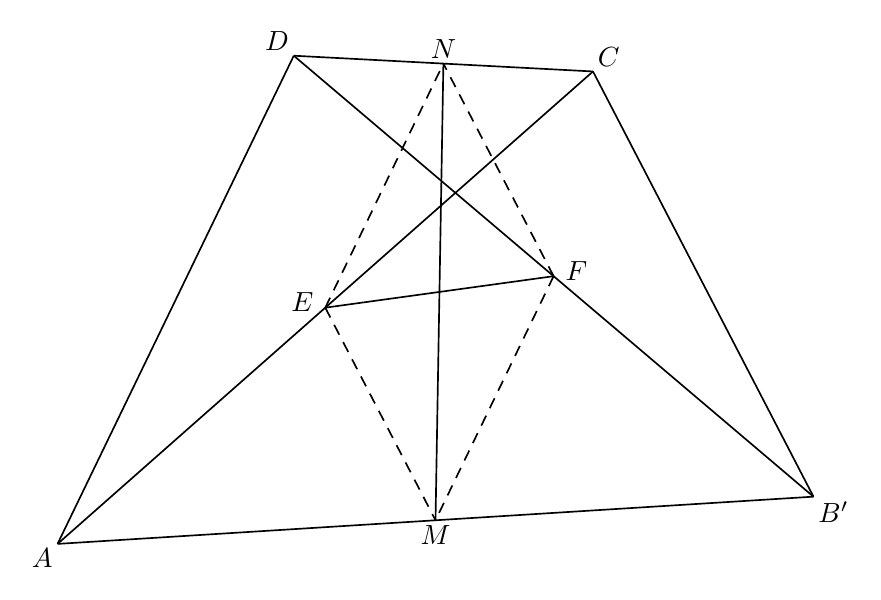
\begin{tikzpicture}[line width=.6pt,font=\normalsize,>=Latex]
  \coordinate (A) at (0,0);
  \coordinate (B) at (9.6,0.6);
  \coordinate (C) at (6.8,6.0);
  \coordinate (D) at (3.0,6.2);
  \coordinate (M) at (4.8,0.3);
  \coordinate (N) at (4.9,6.1);
  \coordinate (E) at (3.4,3.0);
  \coordinate (F) at (6.3,3.4);

  % 四边形四边
  \draw (A) -- (B);
  \draw (B) -- (C);
  \draw (C) -- (D);
  \draw (D) -- (A);

  % 两条对角线（点划线）
  \draw[solid] (A) -- (C);
  \draw[solid] (B) -- (D);

  % 中位线四边形 MFNE 的四边（虚线）
  \draw[dash pattern=on 4pt off 3pt] (E) -- (M);
  \draw[dash pattern=on 4pt off 3pt] (E) -- (N);
  \draw[dash pattern=on 4pt off 3pt] (F) -- (M);
  \draw[dash pattern=on 4pt off 3pt] (F) -- (N);

  % 两线段 EF 与 MN
  \draw (E) -- (F);
  \draw (M) -- (N);

  \node[below left,inner sep=1.5pt] at (A) {$A$};
  \node[below right,inner sep=1.5pt] at (B) {$B'$};
  \node[above right,inner sep=1.5pt] at (C) {$C$};
  \node[above left,inner sep=1.5pt] at (D) {$D$};
  \node[below,inner sep=1.5pt] at (M) {$M$};
  \node[above,inner sep=1.5pt] at (N) {$N$};
  \node[left,inner sep=2pt,xshift=-2pt,yshift=2pt] at (E) {$E$};
  \node[right,inner sep=2pt,xshift=2pt,yshift=2pt] at (F) {$F$};
\end{tikzpicture}
